\documentclass[
	aspectratio=169,	% Modern aspect ratio (TODO: Other ratios not yet supported)
	onlytextwidth,		% Sets totalwidth=\textwidth and therefore e.g. columns won't invade the margins
	t,					% Default vertical alignment of frames and colums at top (default is centered) % Stored in \beamer@centered (\beamer@centeredfalse, \beamer@centeredtrue)
%	handout,			% Create a basic handout of the presentation (removes overlays)
	]{beamer}


%%%%%%%%%%%%%%%%%%%%%%%%%%%%%%%%%%%%%%%%%%
% 1) Load the desired presentation theme
\usetheme[
% Individual options to customize the presentation conforming to the corporate design
hs,					% Change default faculty color set and predefined faculty values: hs or <empty> (default), inw, cb, me, sw, wi, inst (\renewcommand{\insertfacultyname}{Institutname} needed)
faculty=cb,
%	language=english,	% Change language to english (default: ngerman), other languages are possible (see babel-package) but may need further adjustments 
%	toc,				% Adds a ToC slide
	sectionslide,		% Display separate section slides
%	subsectionslide,		% Display separate subsection slides containing section and subsection name
%	smallpagenumber,	% Reduces the size of the page number
%	nototalpages,		% Hides the total number of slide in footline
%	nofacultyicon,		% Hides the faculty icon on title page
colormath=nottext,	% Enables coloring of math text: off or <empty>, full, nottext (default)
%	printhandout,		% Places two slides on a single a4 paper for printing the presentation (beamer class option 'handout' needed)
%	noframesubtitle,	% Disables frame subtitles alltogether and slightly increases frame height
% Additional style options not completely conforming to the corporate design
%	titlepagedate,		% Shows the date on the titelpage
%	fancystyle,			% Enables some fancy styles, that are not part of the corporate design specifications (default: off)
%	progressbar,		% Shows the progressbar in footline (run twice to update progressbar)
]{hsmw} 

%%%%%%%%%%%%%%%%%%%%%%%%%%%%%%%%%%%%%%%%%%
% 2) Specify default fields for presentation and pdf document properties
% Set the title: \title{Long title everywhere} or \title[Short title for footline]{Long title for titlepage}
\title{Evaluierung von KI-basierten Modellen zur automatisierten Schwachstellenanalyse im Rahmen von Penetrationstests}
% Authors (separate multiple author names e.g. with \and for additional space): \author{author for everywhere} or \author[author for footline]{author for titlepage and thankyouslide}
\author[xxx]{xxx}
% Institute (will be prefilled automatically, depending on chosen faculty theme option): \institute{institute for everywhere} or \institute[institute for footline and thankyouslide]{institute for titlepage}
%\institute[institute for footline and thankyouslide]{institute for titlepage}
% Date of presentation (\today or a fixed value): \date{date for everywhere} or \date[date for footline]{date for titlepage}
%\date{\today} % 22. März 2022
% Impressum for thankyou slide (leave one empty if not wanted or needed):
%\email{schildba@hs-mittweida.de} % \email{E-Mail}
%\phone{+49 3727 58-1598} % \phone[Mobile Number]{Telephone Number}
%\office{Haus 8 | Richard Stücklen-Bau | Raum 8-207\newline Am Schwanenteich 6b | 09648 Mittweida} % \office{Office}
%\courseofstudies{Informatik (IF10w1-M)} % \courseofstudies{Course of Studies (Group Number)}
%\additional[Sidebar Text]{Main Text} % Additional information you may want to give (Department, Module, etc.) \additional[Sidebar Text]{Main Text}

%%%%%%%%%%%%%%%%%%%%%%%%%%%%%%%%%%%%%%%%%%
% 3) Use features
% Titlegraphic changes the title page to "wide" (default) if left empty or inserts given image (by file path) and scales to 6.2cm height otherwise:
\titlegraphic{} %\titlegraphic{figures/thankyou.jpg}

%%%%%%%%%%%%%%%%%%%%%%%%%%%%%%%%%%%%%%%%%%
% 4) Add bibliography
% Load the package and options you like, e.g. for recommended ieee style in combination of biblatex and biber:
%\usepackage[backend=biber, bibstyle=ieee, citestyle=numeric-comp, sorting=none, natbib=true, hyperref=true, dashed=false]{biblatex}
% Add your bibliography file(s)
%\addbibresource{literature.bib} 
% Dont forget to use \makebibliography where you want to put it, e.g. at the end of your presentation, after the "normal" slides:
% \appendix
% \makebibliography
% Compile with following command sequence to fully include bibliography: pdflatex, biber, pdflatex, pdflatex

%%%%%%%%%%%%%%%%%%%%%%%%%%%%%%%%%%%%%%%%%%
% 5) Existing macro usage examples

% \appendix is used as end marker for slides (slide numbers and progressbar)
% \makethankyou creates a thank you slide and is used as end marker for slides (progressbar)
% \makebibliography creates one or multiple bibliography slides

% For multiple speakers you can use \setcurrentspeaker{speaker name} or \setcurrentspeaker*{speaker name} prior to the frame
% To reset to the default author, use \resetcurrentspeaker{} or \resetcurrentspeaker*{}
% Starred versions of these macros prepend the word "speaker"

%%%%%%%%%%%%%%%%%%%%%%%%%%%%%%%%%%%%%%%%%%
% 6) Import additional packages you need, (re-)define macros and create a wonderful latex presentation

% You can remove this package - it is only needed for the dummy content
\usepackage{blindtext}







%%%%%%%%%%%%%%%%%%%%%%%%%%%%%%%%%%%%%%%%%%
\begin{document}
	
\begin{frame}{Agenda}
	\begin{enumerate}
		\item Problem \& Motivation \& Ziel der Arbeit
		\item Grundlagen
		\item Methodik
		\item Praxistests \& Ergebnisse
		\item Vergleich \& Bewertung
		\item Fazit \& Ausblick
	\end{enumerate}
\end{frame}


\section{1. Problem \& Motivation \& Ziel der Arbeit}
\begin{frame}{Problem \& Motivation}
	\begin{columns}
		\begin{column}{0.48\textwidth}
			\textbf{Problem:}
			\begin{itemize}
				\item Pentests etabliert, aber teuer \& zeitaufwendig
				\item Fachkräftemangel in IT-Security
				\item Wachsende Angriffsflächen (Cloud, Microservices, DevOps)
			\end{itemize}
		\end{column}
		\begin{column}{0.48\textwidth}
			\textbf{Motivation:}
			\begin{itemize}
				\item Automatisierung \& Beschleunigung
				\item Reduktion menschlicher Fehler
				\item Schnellere Reaktionen auf Bedrohungen
				\item Abfederung Fachkräftemangel
			\end{itemize}
		\end{column}
	\end{columns}
\end{frame}




\begin{frame}{Ziel der Arbeit}
	\textbf{Forschungsfrage:}  
	Inwiefern können KI-gestützte Modelle typische Aufgaben im Pentest unterstützen, beschleunigen oder automatisieren?
	

	\textbf{Ziele:}
	\begin{itemize}
		\item Praxisnaher Bewertungsrahmen
		\item Durchführung realitätsnahe Praxistests
		\item Vergleich von Stärken \& Schwächen
	\end{itemize}
\end{frame}


\section{2. Grundlage}
\begin{frame}{Grundlage 1/3}{Was sind Penetrationstests?}
	\begin{itemize}
		\item \textbf{Definition:} Simulation realer Angriffe auf IT-Systeme
		\item \textbf{Zweck:} Schwachstellen frühzeitig finden \&  bewerten
		\item \textbf{Arten:}
		\begin{itemize}
			\item Black-Box (keine Vorkenntnisse)
			\item Grey-Box (teilweise Infos)
			\item White-Box (vollständige Infos)
		\end{itemize}
	\end{itemize}
\end{frame}


\begin{frame}{Grundlage 2/3}{Pentest-Phasen (BSI-Modell)}
	\centering
	\includegraphics[width=0.85\textwidth]{figures/Phase.png}
	\label{fig:phase}
\end{frame}


\begin{frame}{Grundlage 3/3}{KI im Pentest-Kontext}
	\begin{itemize}
		\item \textbf{Künstliche Intelligenz (KI)}
		\begin{itemize}
			\item Muster erkennen \& Prozesse automatisieren
			\item Unterstützung bei Entscheidungen
		\end{itemize}
		
		\vspace{2mm}
		\item \textbf{Large Language Models (LLMs)}
		\begin{itemize}
			\item Zerlegen komplexer Aufgaben in Einzelschritte
			\item Exploit-Ideen \& Payloads generieren
			\item Automatisierte Dokumentation
		\end{itemize}
		
		\vspace{2mm}
		\item \textbf{Schwächen}
		\begin{itemize}
			\item Halluzinationen (falsche, aber plausible Antworten)
			\item Begrenztes Kontextfenster
		\end{itemize}
	\end{itemize}
\end{frame}


\section{3. Methodik}

\begin{frame}{Welche Tools wurden getestet?}
	
	\begin{itemize}
		\item \textbf{RamiGPT}
		\begin{itemize}
			\item Fokus: Privilege Escalation (Linux/Windows)
			\item Kombination von KI-Logik \& klassischen Tools (LinPEAS, BeRoot)
		\end{itemize}
		
		\item \textbf{PentestGPT (CLI)}
		\begin{itemize}
			\item Open Source (Projekt GreyDGL)
			\item Strukturierte Workflows, textbasiert in der Konsole
		\end{itemize}
		
		\item \textbf{PentestGPT (Web)}
		\begin{itemize}
			\item Kommerziell, anderer Anbieter als CLI-Version
			\item Dialogorientiert, direkt im Browser nutzbar
		\end{itemize}
	\end{itemize}
	\textbf{Alle getesteten Tools nutzen GPT-LLMs}
	
\end{frame}



\section{4. Praxistests: RamiGPT-Privilege Escalation}
% Folie – Grundlagen: Privilege Escalation
\begin{frame}{Was ist Privilege Escalation?}
	\begin{itemize}
		\item \textbf{Ziel:} Unberechtigter Root/Admin-Zugriff
		\item Post-Exploitation-Phase
		\item \textbf{Typische Techniken (nach MITRE ATT\&CK):}
		\begin{itemize}
			\item Exploitation von Systemschwachstellen (T1068)
			\item Missbrauch von Sudo/SetUID (T1548)
			\item Manipulation von Zugriffstokens (T1134)
			\item Nutzung gültiger, privilegierter Accounts (T1078)
		\end{itemize}
	\end{itemize}
\end{frame}

\begin{frame}{RamiGPT – Szenario}
	\begin{columns}
		\begin{column}[T]{.45\textwidth}
			\begin{itemize}
				\item \textbf{Ziel:} Root-Rechte über \texttt{rootbash}
				\item \textbf{Setup:} Ubuntu-VM mit absichtlich fehlerhafter SetUID
				\item \textbf{Testmodi:} Full-AI vs. Halb-automatisch
			\end{itemize}
		\end{column}
		\begin{column}[T]{.55\textwidth}
			\centering
			\vspace{-4mm}
			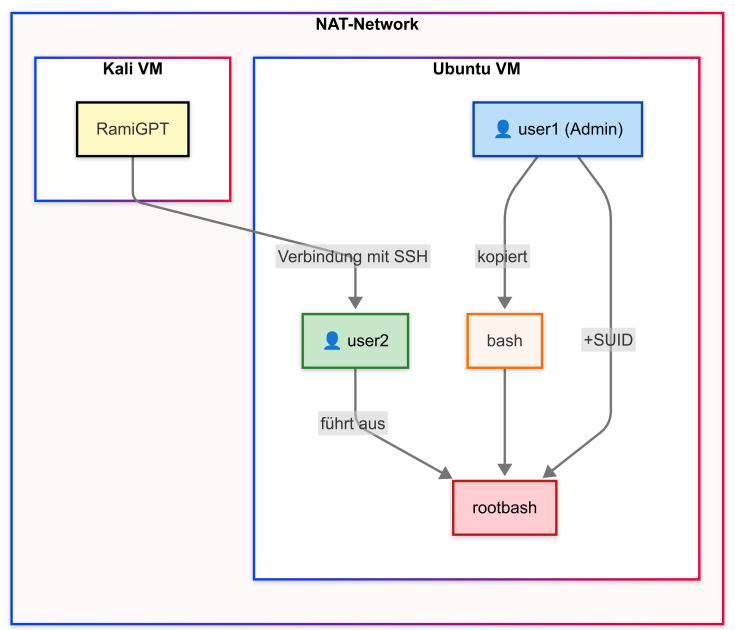
\includegraphics[width=0.9\textwidth]{figures/14.png}
			\label{fig:14}
		\end{column}
	\end{columns}
\end{frame}



\begin{frame}{Full-AI-Modus (Fehlschlag)}
	\begin{columns}
		\begin{column}[T]{.45\textwidth}
			\begin{itemize}
				\item Startet \texttt{sudo}-Befehle
				\item Bleibt bei Passwort hängen
				\item \texttt{rootbash} nicht erkannt
			\end{itemize}
			\textbf{Ergebnis:} Full-AI scheitert
		\end{column}
	\begin{column}[T]{.55\textwidth}
		\centering
		\vspace{-7mm}
		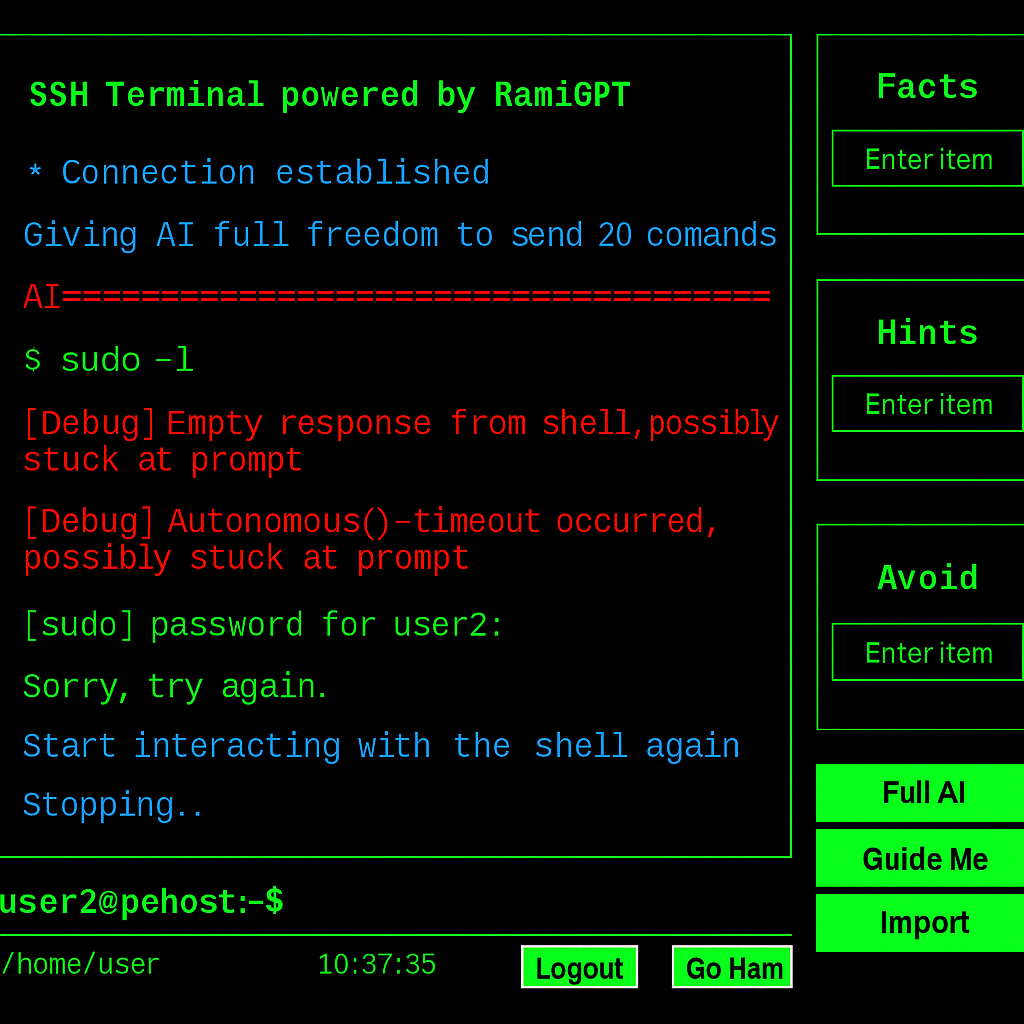
\includegraphics[width=0.8\textwidth]{figures/6.png}
		\label{fig:6}
		\end{column}
	\end{columns}
\end{frame}


\begin{frame}{Halb-automatischer Ablauf (1/2)}
	\begin{columns}
		\begin{column}[T]{.45\textwidth}
			\begin{itemize}
				\item Nutzerhilfe: \texttt{ls} $\rightarrow$ Kontext
				\item RamiGPT findet \texttt{rootbash}
				\item Führt aber nicht selbst aus
			\end{itemize}
		\end{column}
		\begin{column}[T]{.55\textwidth}
			\centering
			\vspace{-8mm}
			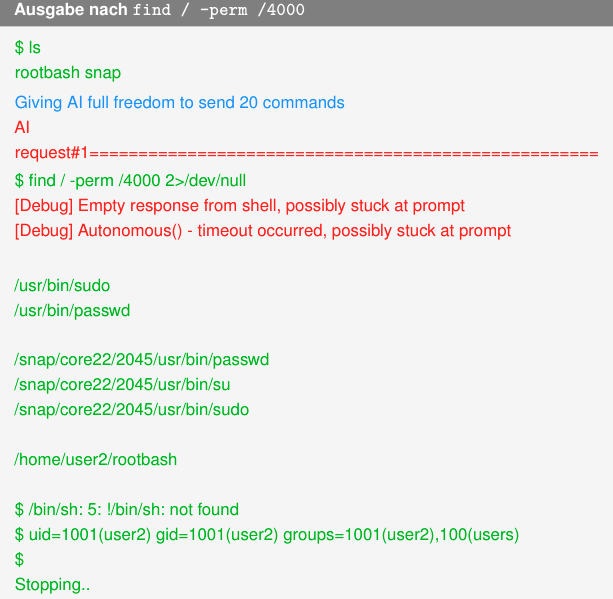
\includegraphics[width=0.8\textwidth]{figures/11.png}
			\label{fig:11}
		\end{column}
	\end{columns}
\end{frame}


\begin{frame}{Halb-automatischer Ablauf (2/2)}
	\begin{itemize}
			\item Nutzer: \texttt{ls -la} $\rightarrow$ Datei erkannt
			\item Tool startet \texttt{./rootbash}
			\item Ergebnis: Root-Rechte (\texttt{uid=0/root})
	\end{itemize}
	\textbf{Fazit:} Erfolg nur mit Nutzerhilfe
\end{frame}


\section{4. Praxistests: PentestGPT (CLI)}

% Folie 4 – Penetrationstests
\begin{frame}{Grundlagen OWASP Top 10 (A01–A03)}
	\begin{columns}
		% Linke Spalte: Text
		\begin{column}[T]{.65\textwidth}
			\begin{itemize}
				\item \textbf{A01:} Zugriffskontrollen umgehen  
				(JWT, IDOR)
				\item \textbf{A02:} Schwache / unsichere Kryptografie
				\item \textbf{A03:} Unsichere Eingaben  
				(SQLi, XSS)
			\end{itemize}		
		\end{column}
		\begin{column}[T]{.3\textwidth}
			\vspace*{-4mm}
			\centering
			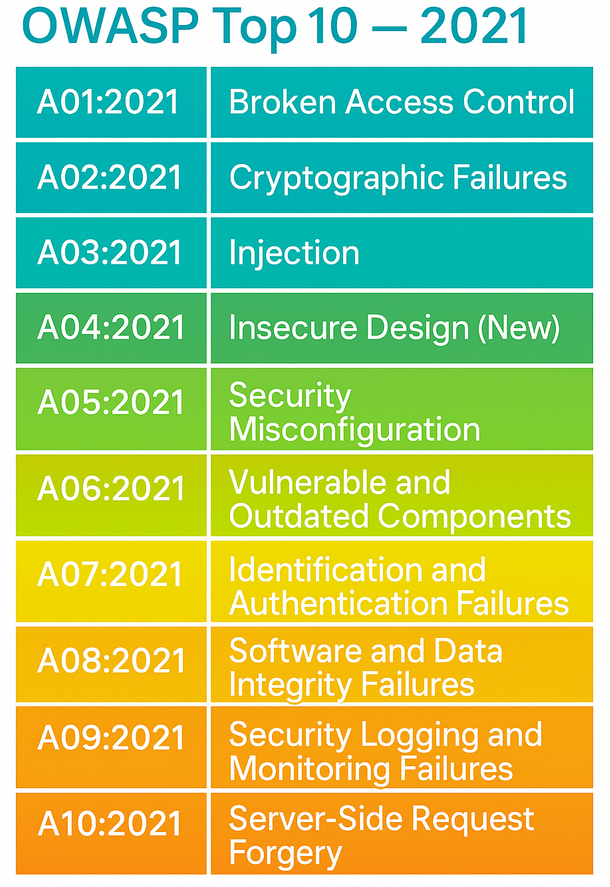
\includegraphics[width=\textwidth]{figures/4.png}
			\label{fig:4}
		\end{column}
	\end{columns}
\end{frame}


\begin{frame}{PentestGPT (CLI) – Szenarien}
	\begin{itemize}
		\item \textbf{Zielsystem:}  
		OWASP Juice Shop (verwundbare Web-App)
		
		\vspace{2mm}
		\item \textbf{Schwachstellen:}  
		A01–A03 OWASP Top 10
		
		\vspace{2mm}
		\item \textbf{Interaktion:}
		\begin{itemize}
			\item Strukturierte Workflows über CLI-Befehle 
			(\texttt{next}, \texttt{more}, \texttt{discuss})
			\item GPT-gestützte Vorschläge, Ausführung durch Nutzer
		\end{itemize}
	\end{itemize}
\end{frame}


\begin{frame}{PentestGPT (CLI) – Szenarien}
	\begin{columns}
		\begin{column}[T]{.4\textwidth}
			\begin{itemize}
				\item \textbf{Zielsystem:}  
				OWASP Juice Shop 
				
				\item \textbf{Schwachstellen:}  
				A01–A03 
				
				\item \textbf{Interaktion:}
				\begin{itemize}
					\item Strukturierte Workflows über CLI-Befehle \\
					(\texttt{next}, \texttt{more}, \texttt{discuss})\\
					\item GPT-gestützte Vorschläge, Ausführung durch Nutzer
				\end{itemize}
			\end{itemize}
		\end{column}
		\begin{column}[T]{.6\textwidth}
			\centering
			\vspace{-4mm}
			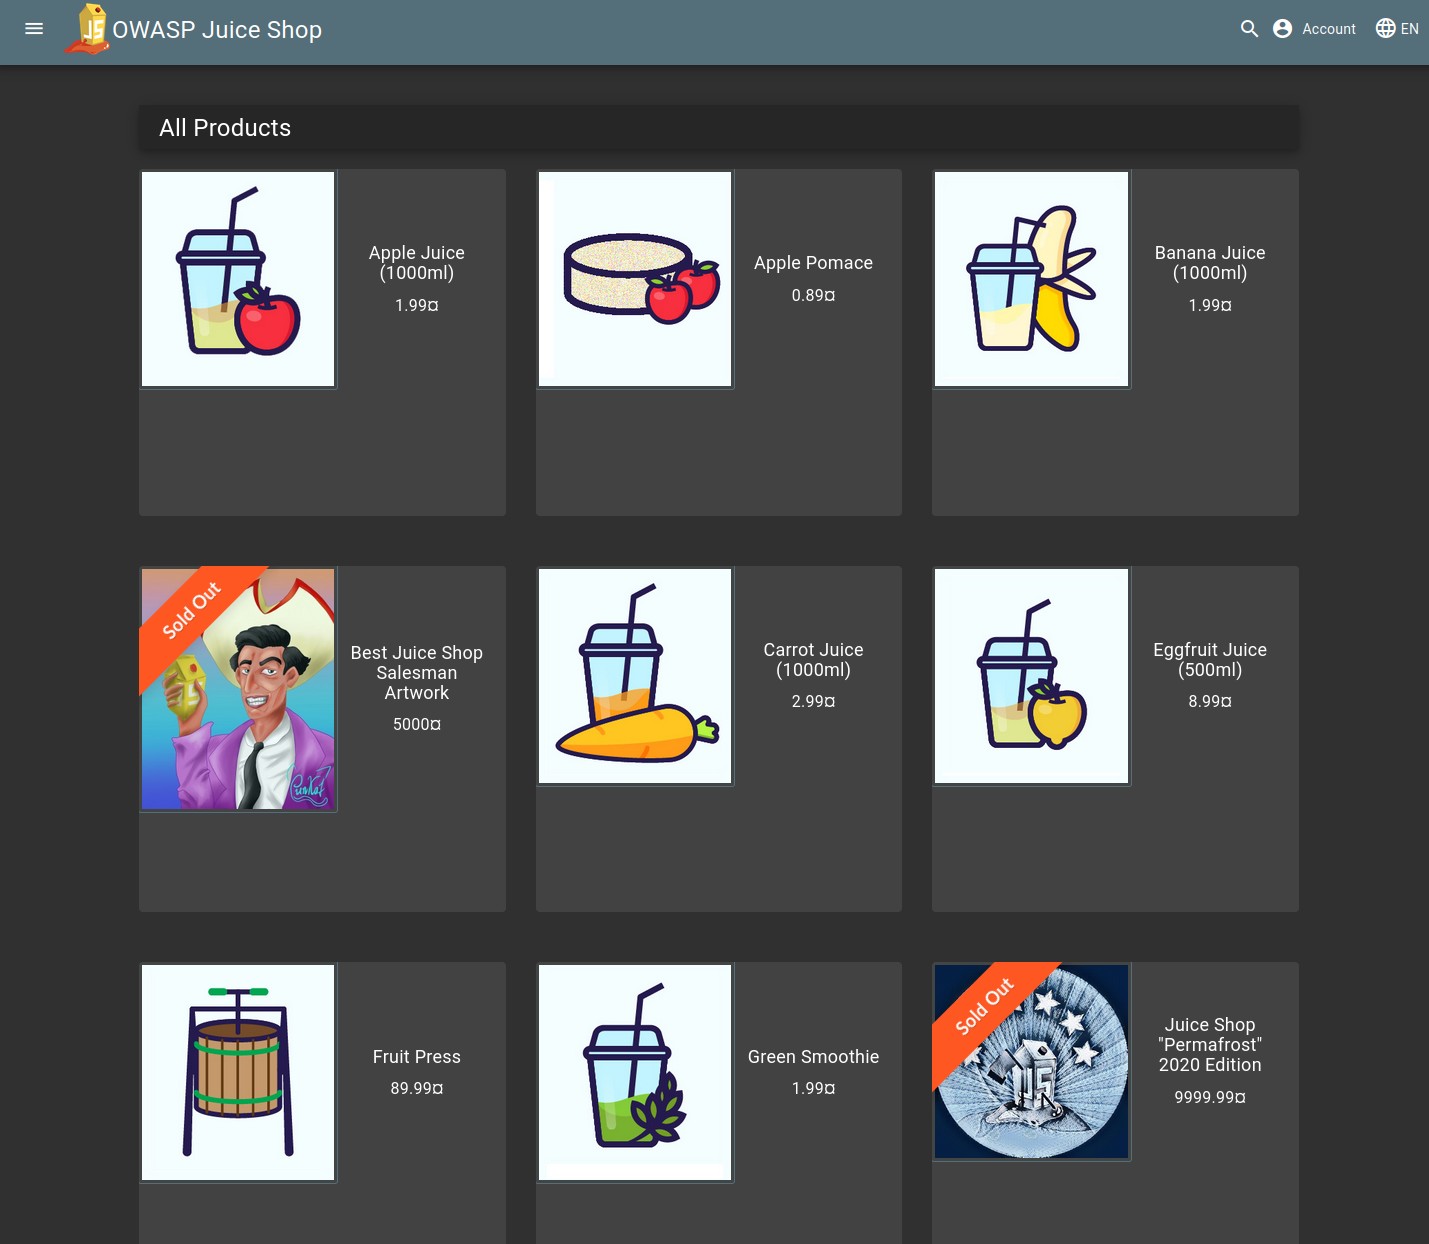
\includegraphics[width=0.75\textwidth]{figures/23.png}
			\label{fig:23}
		\end{column}
	\end{columns}
\end{frame}



\begin{frame}{Test – Exploit-Vorschlag}
	\begin{columns}
		\begin{column}[T]{.4\textwidth}
			\begin{itemize}
				\item Vorschläge für konkrete Exploits (z. B. SQLi)
				\item Liefert fertige Payloads wie \textbf{\texttt{' OR '1'='1}}
			\end{itemize}
		\end{column}
		\begin{column}[T]{.6\textwidth}
			\centering
			
			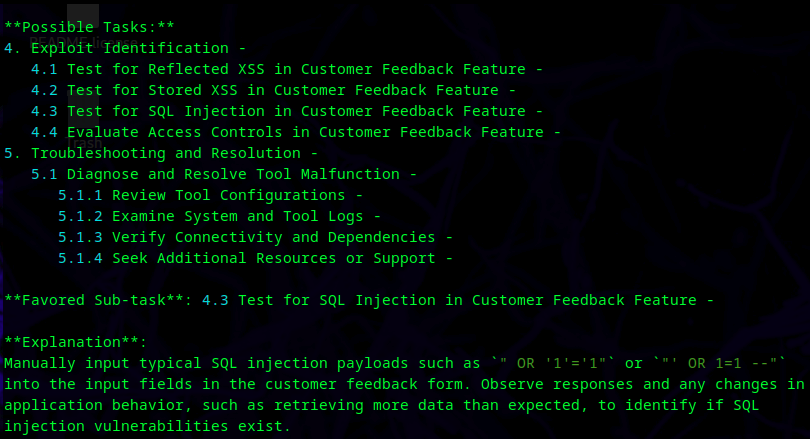
\includegraphics[width=0.9\textwidth]{figures/13.png}
			\label{fig:13}
		\end{column}
	\end{columns}
\end{frame}


\begin{frame}{PentestGPT (CLI) – Ergebnisse}
	\begin{itemize}
		\item \textbf{Stärken:}
		\begin{itemize}
			\item valide Payloads
			\item strukturierte Tests
		\end{itemize}
		
		\item \textbf{Schwächen:}
		\begin{itemize}
			\item keine Automatisierung
			\item Kein Reporting-Export, nur Logfiles
		\end{itemize}
		
		\item \textbf{Fazit:}  
		gutes Assistenztool für Ausbildung \& strukturierte Tests
	\end{itemize}
\end{frame}


\section{4. Praxistests: PentestGPT (WEB)}
\begin{frame}{PentestGPT (Web) – Szenarien}
	\begin{columns}
		\begin{column}[T]{.4\textwidth}
			\begin{itemize}
				\item \textbf{Zielsystem:} OWASP Juice Shop
				\item \textbf{Schwachstellen:} A01–A03 
				\item \textbf{Interaktion:}
				\begin{itemize}
					\item Dialogorientiert (ähnlich ChatGPT)
					\item Prompts in natürlicher Sprache (DE/EN)
					\item Ad-hoc-Analysen direkt im Browser
				\end{itemize}
			\end{itemize}
		\end{column}
		\begin{column}[T]{.6\textwidth}
			\centering
			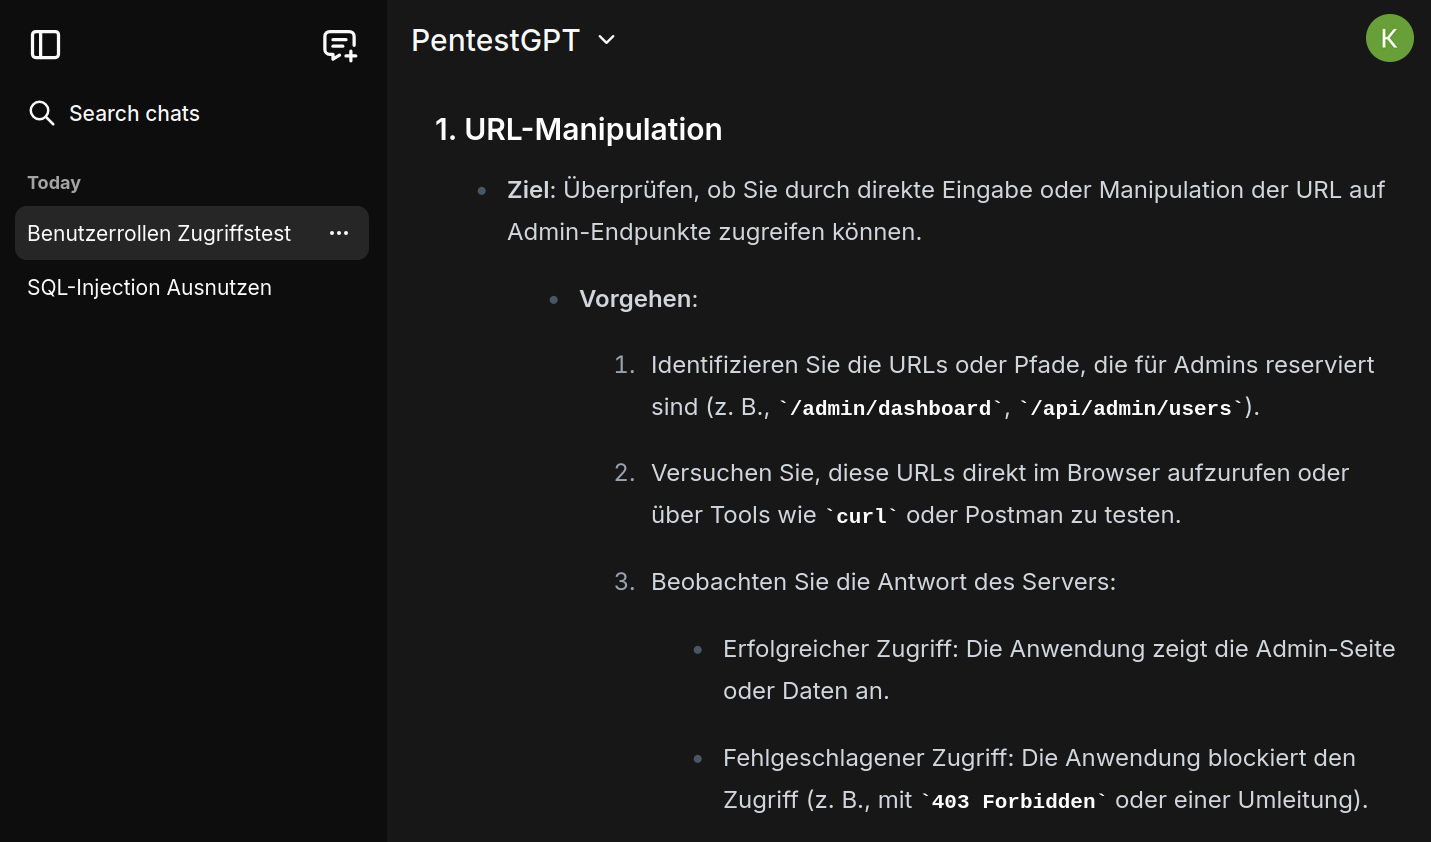
\includegraphics[width=0.9\textwidth]{figures/22.png}
			\label{fig:22}
		\end{column}
	\end{columns}
\end{frame}


% Folie – PentestGPT (Web): Ergebnisse
\begin{frame}{PentestGPT (Web) – Ergebnisse}
	\begin{itemize}
		\item \textbf{Stärken:}
		\begin{itemize}
			\item Schnelle \& präzise Antworten (inkl. Exploits)
			\item Keine Installation, einfache Bedienung
			\item Kontextsensitiv (Deutsch/Englisch)
		\end{itemize}
		
		\item \textbf{Schwächen:}
		\begin{itemize}
			\item Keine Automatisierung
			\item Kein Reporting (nur Chat)
			\item Voller Funktionsumfang kostenpflichtig
		\end{itemize}
		
		\item \textbf{Fazit:}  
		Praktisch für schnelle Analysen, weniger für strukturierte Tests
	\end{itemize}
\end{frame}



\section{Vergleich \& Evaluierung der Tools}
\begin{frame}{Vergleich der Tools}
	\centering
	\textbf{Bewertung nach 6 Kriterien (0–2 Punkte, max. 12):}
	
	\vspace{5mm}
	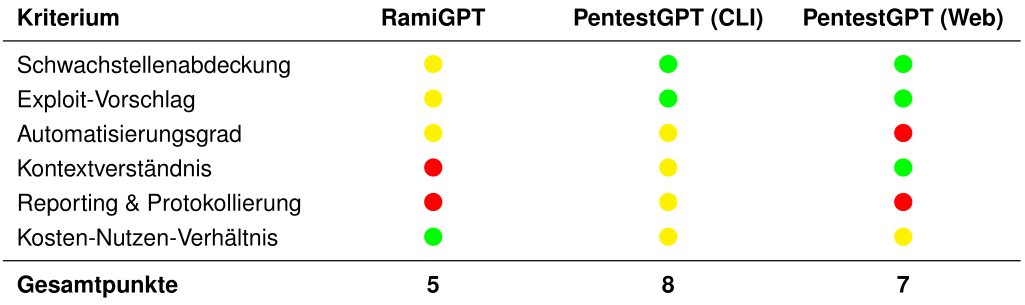
\includegraphics[width=\textwidth]{figures/20.png}
	\label{fig:20}
\end{frame}

		
\begin{frame}{Zusammenfassen}
	\begin{itemize}
		\item \textbf{RamiGPT} $\rightarrow$ unreif, nur für Privilege Escalation interessant
		\item \textbf{PentestGPT (CLI)} $\rightarrow$ methodisch klar, gute Payloads, aber rein manuell
		\item \textbf{PentestGPT (Web)} $\rightarrow$ schnell \& flexibel, aber limitiert ohne Automatisierung
	\end{itemize}
\end{frame}


\section{Fazit \& Ausblick}
% Folie – Fazit
\begin{frame}{Fazit}
	\begin{itemize}
		\item \textbf{KI = Unterstützung, kein Ersatz}  
		$\rightarrow$  menschliche Expertise bleibt unverzichtbar
		
		\item \textbf{Nutzen:}
		\begin{itemize}
			\item Effizienzsteigerung bei Routineaufgaben
			\item Hilfreich für Ausbildung \& strukturierte Analysen
			\item Schnelle Proof-of-Concepts möglich
		\end{itemize}
		
		\item \textbf{Grenzen:}
		\begin{itemize}
			\item Keine vollständige Automatisierung
			\item Ergebnisse nicht immer reproduzierbar
			\item Eingeschränktes Kontextverständnis
		\end{itemize}
	\end{itemize}
\end{frame}





% Folie – Ausblick
\begin{frame}{Ausblick}
	\begin{itemize}
		\item \textbf{Integration in DevSecOps}  
		$\rightarrow$  KI-gestützte Tools als Teil kontinuierlicher Sicherheitsprozesse
		
		\item \textbf{Technische Weiterentwicklung}  
		$\rightarrow$  Größere Kontextfenster \& verbesserte Modelle  
		$\rightarrow$  Retrieval-Augmented Generation (RAG) für aktuelles Wissen
		
		\item \textbf{Anwendung in der Ausbildung}  
		$\rightarrow$  KI als interaktiver Trainingspartner  
		$\rightarrow$  Unterstützung beim Erlernen von Angriffstechniken \& Abwehrmaßnahmen
		
		\item \textbf{Langfristige Perspektive}  
		$\rightarrow$  KI erweitert klassische Pentests  
		$\rightarrow$  Richtung: skalierbare \& adaptive Sicherheitsprüfungen
	\end{itemize}
\end{frame}








%
	\appendix
	\appendix
	\section*{Literatur}
	
	\begin{frame}[allowframebreaks]{Literatur}
		\begin{thebibliography}{9}
			\bibitem{bitkom2023}
			Bitkom (2023): \\
			Mangel an IT-Fachkräften droht sich zu verschärfen. \\
			\url{https://www.bitkom.org/Presse/Presseinformation/Mangel-an-IT-Fachkraeften-droht-sich-zu-verschaerfen}
		\end{thebibliography}
	\end{frame}
	
	\makethankyou
%	\makebibliography
%
%	\section{\appendixname}
%
%	\begin{frame}{Zusätzliche Folien}{Der Anhang zählt nicht mit zu den regulären Folien}
%		\blindtext
%	\end{frame}

\end{document}
